\documentclass{article}

\usepackage[utf8]{inputenc}
\usepackage{amsmath}
\usepackage{float}
\usepackage[top=1.5cm,bottom=1.5cm,left=1.5cm,right=1.5cm]{geometry}
\usepackage{graphicx}
\usepackage{listings}
\usepackage{color}
\definecolor{mycolor}{gray}{0.95}
\lstset{language=Bash,breaklines = true, backgroundcolor=\color{mycolor}}
\usepackage[usenames,dvipsnames]{xcolor}
\usepackage{multicol}

\begin{document}
\begin{center}
{\Large \textbf{Utilización del Arduino para controlar motores de paso por medio del flasheo de GRBL}}\\
\vspace{0.3cm}
\textit{Alfredo Ricci, Juan Andrés Urrea}
\end{center}
\begin{multicols}{2}
\textbf{Resumen- Este informe busca mostrar la totalidad del procedimiento realizado para configurar un computador y un arduino como controladores para motores de paso. Se centra especialmente en la instalación del software necesario tanto en su utilización una vez esto se completa. De esta forma, explica el procedimiento de instalación y configuración, sirviendo a la vez como un tutorial para repetir este procedimiento.}

{\centering \section{Introducción}}
Dada la necesidad de tener un conocimiento previo del manejo tanto manual como automatizado de los mtores utilizados para el proyecto \textbf{Mechanical Scanner}, se ideó la estrategia de reproducir esta situación a pequeña escala, usando motores de paso para luego conectarlos a un Arduino flasheado con GRBL y aprender, desde cero, los procesos necesarios para transmitir órdenes de trayectorias desde un computador hasta los motores de paso utilizados. De esta forma, la construcción exitosa de este montaje y la capacidad de controlar detalladamente estos dispositivos por medio de un manejo apropiado del software permitirá obtener este conocimiento previo a la llegada y utilización del \textbf{Mechanical Scanner}.

{\centering \section{Montaje Utilizado}}
DESCRIBIR MONTAJE CON FOTO Y TEXTO.

{\centering \section{Manejo de Software}}
{\centering \subsection{Instalación de Software Utilizado}}
Antes de la explicación detallada acerca del proceso de instalación, se enuncian a continuación los diferentes programas y software utilizados:
\begin{itemize}
\item \textbf{GRBL}\\
\begin{itemize}
\item Versión: 0.8
\end{itemize}
GRBL es un controlador de movimiento disponible para funcionar con Arduino, escrito enteramente en \textit{C}, que sirve como alternativa al control por puerto paralelo. Este software permite utilizar archivos escritos en \textit{GCode} para diseñar trayectorias a seguir, de manera que estos se convierten en instrucciones para el Arduino, por medio de la instalación de GRBL, que luego son enviadas a la tarjeta controladora CNC.

\item \textbf{Arduino UNO}\\
\begin{itemize}
\item Versión 1.6.5
\end{itemize}
Software que funciona como interfaz para controlar el dispositivo arduino desde un computador. Puede instalarse directamente desde la página web de Arduino. Software programado en Java, permite la creación de código que luego es subido directamente al dispositivo Arduino.

\item \textbf{GCode Universal Sender}\\
\begin{itemize}
\item Versión: 1.0.8
\end{itemize}
Software escrito en Java que funciona como complemento para GBRL como intérprete de código G que puede ser enviado directamente al Arduino para ser interpretado como trayectoria. Permite, además de esta alternativa automatizada, un control manual por medio de botones que indican movimiento en cada eje, lo que es traducido luego a código G y enviado también al Arduino.

\end{itemize}
\begin{center}
\textbf{Instalación del Software Requerido}
\end{center}
Una cez se sabe cual es el software requerido, se presenta ahora el proceso detallado de instalación de estos. Cabe notar que el proceso mostrado a continuación se realizó tanto en Linux como en Mac. Esto con la finalidad de utilizar los procedimientos más sencillos que ofrece cada sistema operativo. Para este caso, el flasheo de GRBL al Arduino se realizó desde Linux, mientras que la construcción y envío de GCode al Arduino se realizó desde Mac. Estas diferencias se enunciarán en cada paso.

\begin{enumerate}
\item \textbf{Revisión de Librerías de Instalación Linux}\\
Cuando se trabaja con Linux, especificamente la distribución Ubuntu 14.04 "Trusty", se debe realizar una verificación de librerías que permiten la instalación correcta de paquetes. Dicho proceso se puede realizar con los siguientes comandos de instalación en la terminal. En caso de que ya se encuentren actualizadas, en la terminal esto será notificado. En caso de que no, se instalarán.
\begin{lstlisting}
sudo apt-get install ruby
sudo apt-get install avrdude
\end{lstlisting}

\item \textbf{Descargar GRBL y Flashearlo}\\
Ahora, es necesario descargar todo lo relacionado a GRBL. Esto se puede realizar desde GitHub, en el enlace [1]. Para hacer esto, se recomienda, si es que es la primera vez que se trabaja con esta herramienta, seleccionar la opción \textbf{Download Zip} en la parte derecha de la página.
\begin{figure}[H]
\centering
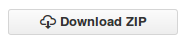
\includegraphics[width=0.3\textwidth]{BotonDescarga.png}
\label{fig:Boton}
\end{figure}

El archivo zip descargado debe luego ser descomprimido en una carpeta cuya localización resulte fácil de recordar. Debido a como está en GitHub, el archivo descargado se llamará \textbf{grbl-edge}. Para continuar este procedimiento, se abre ahora la carpeta recién descargada, buscando el archivo llamada \textbf{Makefile}, el cual debe ser después abierto con un editor de texto de preferencia personal, en este caso \textbf{Gedit}, editor de texto predeterminado de Ubuntu.

\begin{figure}[H]
\centering
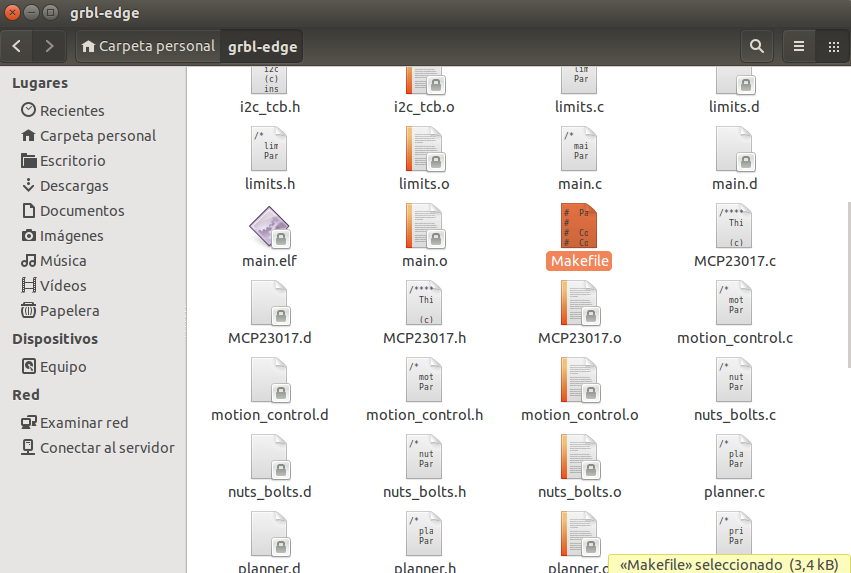
\includegraphics[width=0.4\textwidth]{Carpeta.png}
\label{fig:Carpeta}
\end{figure}

Una vez abierto este archivo, se busca la línea que empieza por la palabra \textit{PROGRAMMER}, para reemplazarla por lo siguiente:
\begin{lstlisting}
PROGRAMMER = -c stk500v1 -P /dev/ttyACM0 -b 115200 
\end{lstlisting}
El archivo luego debe guardarse para actualizar y aplicar los cambios realizados. Una vez se hace esto, se debe abrir una terminal nueva. Esto para aprovechar las ventajas de control que esta aplicación ofrece. Desde esta se debe acceder a la carpeta \textbf{grbl-edge} creada anteriormente. Aunque la apariencia de la terminal depende sustancialmente de la configuración en cada equipo, para este caso específico se obtiene la siguiente ventana:

\begin{figure}[H]
\centering
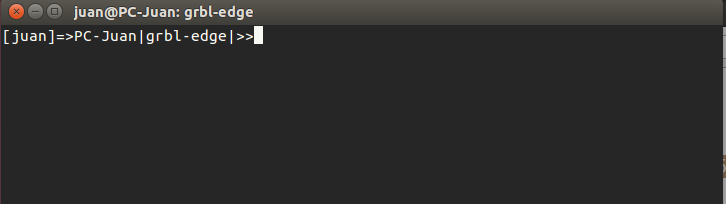
\includegraphics[width=0.45\textwidth]{Terminal.png}
\label{fig:Carpeta}
\end{figure}

Una vez dentro de este entorno, se utiliza las siguientes líneas de código, para inicializar el archivo \textbf{make} dentro de la carpeta.
\begin{lstlisting}
sudo make clean
sudo make
\end{lstlisting}
Realizar esto causará que aparezcan varias notificaciones en la terminal, las cuales sirven únicamente para informar de los procesos completados. Para finalizar este procedimiento, solo resta flashear GRBL al Arduino. Para hacer esto, se debe conectar el Arduino al computador en uso. Luego de hacer esto, se ejecuta en la terminal la siguiente línea de código.
\begin{lstlisting}
sudo make flash
\end{lstlisting}
Esta línea instalará GRBL en el arduino, tras de lo cual se puede desconectar del computador y usar como controlador de movimiento de ahora en adelante.

\item \textbf{Descargar GCode Universal Sender}\\
Para descargar este programa, se recurre de nuevo a GitHub, donde está guardado todo lo relacionado a este software, disponible en [2]. Para comenzar, se descarga la última versión estable disponible. Para Linux y Windows, esta es la versión 1.0.8, mientras que para Mac es la versión 1.0.7. Esto se hace por medio de los links de descarga dados en la sección de información de la página.

\begin{figure}[H]
\centering
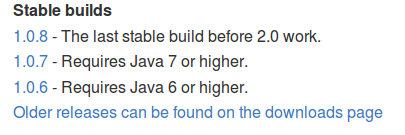
\includegraphics[width=0.4\textwidth]{GCode.png}
\label{fig:Carpeta}
\end{figure}

Dependiendo de en qué sistema operativo se esté trabajando, la manera de ejecutar este programa será diferente. Para este caso, con Ubuntu, se debe utilizar la terminal para ejecutar el archivo \textbf{.jar} dentro de la carpeta descargada, usnado la siguiente línea de código:
\begin{lstlisting}
./UniversalGcodeSender.jar
\end{lstlisting}

\begin{figure}[H]
\centering
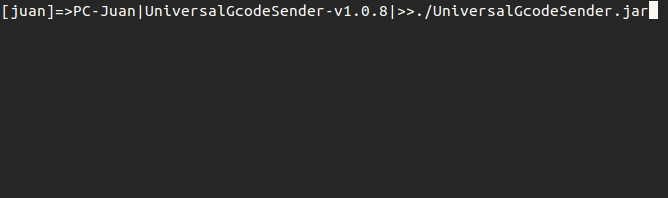
\includegraphics[width=0.45\textwidth]{Sender.png}
\label{fig:Carpeta}
\end{figure}
 

\end{enumerate}
\end{multicols}
\end{document}